\chapter{测试驱动开发} % Introduction chapter suppressed from the table of contents

开发人员问:为什么要这么做?写完程序后,然后再写测试用例,不是更正常吗?

\hypertarget{ux4e3aux4ec0ux4e48ux6211ux4eecux8981ux6d4bux8bd5ux9a71ux52a8ux5f00ux53d1}{%
\subsection{为什么我们要测试驱动开发}\label{ux4e3aux4ec0ux4e48ux6211ux4eecux8981ux6d4bux8bd5ux9a71ux52a8ux5f00ux53d1}}

\textbf{精益}是敏捷中很核心的概念。最近发生的一件事帮我回答了以上问题,也让我体会到TDD与精益的概念是如何协同的。

我有一位拥有几十年电机工程经验的老同学,李先生,他在对Linux的研究方面一直都很有兴趣,这几年又开始玩树莓派,目前他对此非常精通。

最近我找到他,希望在树莓派上安装 Ipython, Jupyter Notebook
等开源应用软件。一直以来,李先生的理念就是尽量用最简单、最轻易的方法去解决客户的问题,而不浪费资源。

例如,当我在三年前开始尝试建立 wiki
服务器给客户使用的时候,他就建议我用树莓派来建:\\
他说:''树莓派不仅省电而且快,也不知道你这个概念是否持久,我不会浪费时间------在大型服务器上安装
Linux +Mediawiki ,如果你觉得这(树莓派)可以,
便继续用。如果觉得它性能不够了,下一步我帮你换更大型的服务器。''

%\href{文件:树莓派2.jpg}{300px}

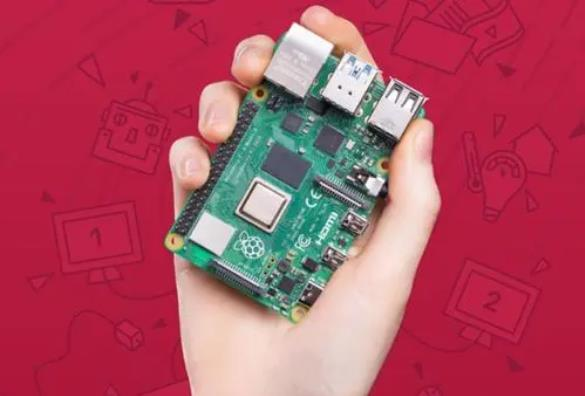
\includegraphics[width=10cm]{树莓派2.jpg}

---直到现在, 已经7 年了,我们一直还是继续用 c
来协助评估(树莓派从原来的Pi2,4G内存,现在已经是P4,4G内存),已经有超过80多个客户在使用了,这证明他的思路是对的。

回到我刚才说要安装 Jupyter Notebook
,他安装好那个程序包后,一直没动。我问他什么原因?他说:他说:``
很简单,我不熟悉软件工程,也不懂如何测试。
肯定要找你测试一下,我才知道有没有做错?避免无谓的返工。''

所以我们就约好周日我回到到办公室跟他远程测试。

李先生打开树莓派后,我用VNC客户端进入他的树莓派,打一些最基本的 Ipython
指令,验证没问题。

下一步我要跑一些比较复杂的、要用到 Pandas 包的 Python
程序,却发现还没有安装Pandas包。他马上到网上去找安装介质以及树莓派如何安装
PANDAS 的方法。
处理好后,我再跑对应的程序,都跑通了,包括之前跑过的指令。前后两个小时,按本来计划,测试成功。

我回想一下,其实他的思路就是精益。用有限的资源、以最低的投入,达到客户要求,不多做。每当李先生做完一步,如果没有通过测试,就不会浪费时间走下一步------这也是精益和测试驱动开发的原理。

\hypertarget{ux6bcfux5c0fux6b65ux9a8cux8bc1}{%
\subsection{每小步验证}\label{ux6bcfux5c0fux6b65ux9a8cux8bc1}}

很久以前,工程类的本科生都要在最后一年做个毕业项目。当时,导师建议我们尝试参考一些常用的语言发声算法,在专门做信号处理的芯片上写程序,读出一些英文字或句子(与现在不同,当时这项技术还没有成熟,很多大学还在研究),虽然我预计有不小的技术难度,但在当时觉得这很先进,所以很感兴趣,便与另一位同学合作,开始制定项目计划。

我们很努力,全情投入,一方面要研究语言发声的算法,还要并行设计电子线路和软件等。我们用了
2、 3
个月的时间做了整个电子线路板的硬件,同时还设计了整个软件架构,并使用计算机模拟,验证每个字实现算法后的发声效果,因为最后一年课程很多,时间过得很快,从9月开始准备一直到次年3月,软硬件的设计与开发终于都完成了,但是不知道什么原因就是没有声音,更不要说能读出一些字和句子了,最后项目以失败告终。

在这之前的一年,我有幸在大学的第三年进入大东电报局实习(当时香港的所有国际通讯都是经过大东),在我实习的部门正如火如荼地开发一套新的电脑系统以取代本来基于UNIVAC的电报系统,总工程师让我用半年时间,在一个微机上编程,做一个系统,以从那些电脑上收集重要信息,如果发现异常就警报。头三个月都是花精力做整个系统设计,也买了一些展示电子版,准备用来展示,但由于经验不足,半年后最终什么都展示不出来。

到了2000年,在我兼读软件工程硕士课程时,开始接触到敏捷开发,才了解到两次项目失败的主因:不应该花大量时间去做前期设计------希望有一个完美的设计,而是应该一步一步迭代,先做一些最基本的简单功能,逐步优化。例如,在我的毕业项目中,应该先做出最基本的硬件、软件,起码能够发出声音,因为没有前人做过,整个项目是从未做过的实验。

敏捷大师Dave Thomas 先生在2015 演讲里提出敏捷软件开发的核心是:

\framebox{%
\begin{minipage}[t]{0.97\columnwidth}\raggedright
\begin{enumerate}
\tightlist
\item
  向你的目标迈出一小步
\item
  从反馈调整你的理解
\item
  重复
\end{enumerate}

\begin{itemize}
\tightlist
\item
  当两种或以上选择的价值大致相同时,选一条让未来更容易修改(软件)的路径
\end{itemize}

Agile Software Development:

\begin{enumerate}
\tightlist
\item
  Take a small step towards your goal\\
\item
  Adjust your understanding based on what you learned\\
\item
  Repeat\\
\end{enumerate}

\begin{itemize}
\tightlist
\item
  When faced with two or more alternatives that deliver roughly the same
  value,take the path that makes future change easier\\
\end{itemize}

\begin{description}
\item[]
\begin{description}
\tightlist
\item[]
(Source: Mr Dave THOMAS, 2015 goto)
\end{description}
\end{description}\strut
\end{minipage}}


这些经历让我体会到为什么我们在写程序时,必须先想一下该怎么测试?

%\hypertarget{ux7528tddux5f00ux53d1ux7a0bux5e8f}{%
%\section{用TDD开发程序}\label{ux7528tddux5f00ux53d1ux7a0bux5e8f}}

\hypertarget{ux6bcfux5c0fux6b65ux9a8cux8bc1}{%
\subsection{用TDD开发程序}\label{ux6bcfux5c0fux6b65ux9a8cux8bc1}}

如果希望在软件开发过程中用 TDD,但又不清楚是什么回事,可先看看Robert
MARTIN的保龄球例子(例如搜索``Rober MARTIN TDD保龄球")\\
如果想了解如何用 TDD 开发 Web 程序,则可参考 Percival 的"TDD with
Python",作者以Selenium做WEB功能测试,配合 Python 做单元测试,加上
Django
的引擎,介绍如何先写功能测试,从客户角度来测试不通过,然后再深入以代码语句思路写单元测试,不通过,再针对单元测试写程序,逐步完成,最后通过功能测试。

%\href{文件:测试.jpg}{400px}

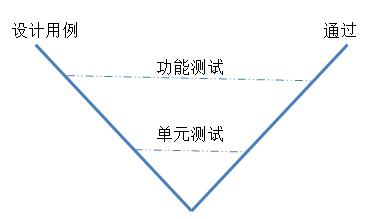
\includegraphics[width=10cm]{测试.jpg}

原则是按部就班地开发,每一步都有单元测试来验证,以避免写了一大堆复杂程序,却无法验证。

程序员问:为什么我们要针对这么小的部分都做单元测试?

答:

\begin{enumerate}
\tightlist
\item
  小的单元测试容易写,比较简单,不会花费很多时间
\item
  因为任何程序都会按时间变化,越来越复杂,有了单元测试,后面的测试就有依据,知道改动是否出错,没有单元测试的话,就没有信心去改程序,不知道是否没问题。
\end{enumerate}

\begin{description}
\item[]
\begin{description}
\tightlist
\item[]
(和我们工程的概念一样,把工程细分,每个子系统都要确保质量达标,尽量找出缺陷,才进行下一步。)
\end{description}
\end{description}

网上有关于是否要TDD的争论:

\begin{itemize}
\tightlist
\item
  一派是坚持要先写测试用例,再写编码
\item
  另一派觉得TDD太多余,如果功能测试做得全,也不一定要有单元测试
\end{itemize}

这个争论让我想起这段时间教ACP敏捷管理的一个原则,叫“守 破 离”。

\hypertarget{ux5b88-ux7834-ux79bb}{%
\subsubsection{守 破 离}\label{ux5b88-ux7834-ux79bb}}

英文翻译成 ``Shu -- Ha -- Ri '' 意思是学习合气道,要先从基本功出发
(守),按规则一步一步做

当你理解以后,就能融会贯通 (破),融合管理到一定境界就是大师级了
(离)。

像宫本武藏(江户时代著名剑术家)一样,一生赢了六十多场决斗,然而到了晚年,他在《五轮书》中总结,不要局限于某种刀法,最重要是抓住原理。

敏捷大师 Mr Cockburn 有一次到企业做 Class-responsibility-collaboration
(CRC) card 咨询培训,因为他很熟悉 CRC 方法,他觉得只要有助于面向对象(OO)
设计,不一定要按原本的方式,可以简化。但学生都不熟悉,一直在问``请你告诉我们从头到尾,每一步如何做,我们照着做''大师没办法,最终按最原始的方法,一步步来教如何去做,学生才能懂,这是守破离的``守''。

TDD测试驱动开发也一样,把TDD看成``守'',当没有概念的时候,还是要从最基本的概念入手,我们每个程序都应该有测试,所以自然的顺序是先写测试用例,再写代码,这也能更好地帮助你理解程序的功能。

所以TDD就是做好程序基本功的基础,当你已经掌握这些基础了,就可以灵活处理,可能不一定要每次先写测试用例,但底线是每个代码都要有单元测试。

但是有些人觉得,只要有功能测试,单元测试可以不做。

功能测试是黑盒测试,从客户的角度测试总体功能,无法真正判断代码是否正确,反过来,单元测试是白盒测试,从代码的功能角度,验证代码是否正确,所以功能测试是不能替代单元测试的。尤其是当代码有功能上的变化时,就更需要有单元测试来验证这些改动是否有误,所以单元测试的复用率非常高。

大家正在越来越多地使用自动集成工具,如果有单元测试,那么每天的自动集成就不仅仅是看编译是否通过,还需要通过单元测试,才能更好地保证代码质量,这就是很有效率的回归测试。(归测试:为避免因代码修改,导致原先通过的测试不通过,所以之前通过的测试用例也要从跑。如果手工测试,为了节省测试时间,只从跑部分重要测试,但如果自动化,就可以轻松地从跑所有测试用例。)

\hypertarget{ux5355ux5143ux6d4bux8bd5ux4e0etddux7684ux597dux5904}{%
\subsection{单元测试与TDD的好处}\label{ux5355ux5143ux6d4bux8bd5ux4e0etddux7684ux597dux5904}}

上周在杭州跟一位资深的开发主管对话,他回国前在日本工作了接近10年,他说很佩服日本注重开发质量,例如很注重单元测试,所以回国后在团队严格要求要有单元测试。

我问:现在有很多静态代码检测,为何还要单元测试。

他答:目的不同,静态代码检测只是用过去的历史经验去检查常见的语法、命名问题,但如果是设计本身的逻辑问题就无法查出。
以他多年的经验,必须通过单元测试才有信心确认这个程序是否正常,单靠集成测试、功能测试是无法确保程序的每一部分都是正常的。所以他严格要求团队,代码经过检验后(自动静态检验或代码走查),还必须做单元测试才能进入下一步的集成、系统测试。

单是靠集成测试、功能测试是无法确保程序每一部分都正常。

他还说TDD 有三点好处:

\begin{enumerate}
\tightlist
\item
  让开发人员在编码前去理解设计和需求
\item
  让开发人员知道代码可验证性的重要
\item
  强迫开发人员主动与设计和需求人员沟通,否则无法设计出单元测试用例
\end{enumerate}

但TDD对团队成员素质要求较高

%\textbf{Reference:}\\

%\hypertarget{ux6bcfux5c0fux6b65ux9a8cux8bc1}{%
%\subsection{Reference:}\label{ux6bcfux5c0fux6b65ux9a8cux8bc1}}

\hypertarget{ux9644ux4ef6}{%
\section{Reference:}\label{ux9644ux4ef6}}

1.Percival, Test Driven Development with Python 2/e

2.Martin R.C., Agile software development - principles, patterns, and
practices





